\section{Examples}
\subsection{A simple case}
The first example we are going to report is very simple but quite instructive.
We simulated a data sample cointaining two classes of event with Gaussian
signal distributions with different mean values and same width.

In Fig.~\ref{fig:Gaus2} the simulated detector responses and the amplitudes
functions derived in such a case a reported. As it can be noted the amplitudes
$\psi_{i}$ are constructed in order to garantee orthogonality with the $p_{k}$
functions for $i \neq k$. In the same figure the bayesian probabilities,
$P_{i}(S)$, are reported as well for a choice of the prior probabilities of
$C_{1}=0.7$ and $C_{2}=0.3$. It is worth to note that the asymmetric behavior
visible in the Bayesian probabilities is due to the asymmetric values of the
abundances. By construction the $P_{i}(S)$ distributions has to respect the
condition:
\begin{equation} 
\label{Sec3:BayesCond}
Cont. (1\rightarrow 2) = \int C_{1} p_{1}(S) P_{2}(S) ds = \int
C_{2} p_{2}(S) P_{1}(S) ds = Cont. (2\rightarrow 1),
\end{equation}
to guarantee a symmetric flux of type-1 event contaminating type-2 class and 
{\it vice versa}.

\begin{figure}[!htb]
\centering
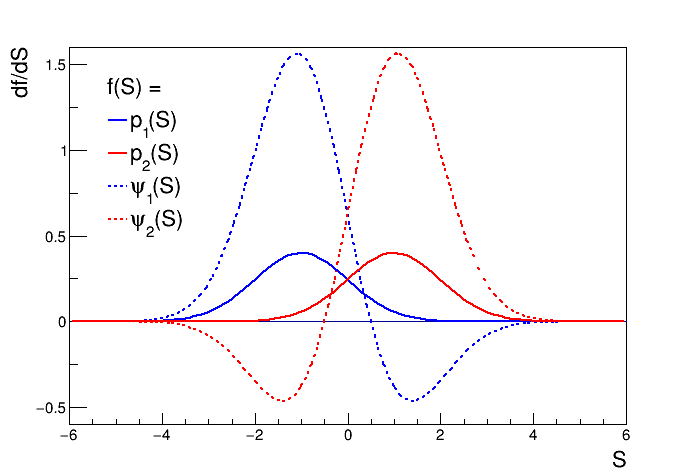
\includegraphics[width=0.7\textwidth]{../png/figGaus2.png}
\caption{Two Gaussian detector responses ($\Delta_{12} = 2$) and relative
  $\psi(S)$ amplitudes. The Bayesian probabilities were computed for a choice
  of the prior probabilities of $C_{1}=0.7$ and $C_{2}=0.3$.}
\label{fig:Gaus2}
\end{figure}

This is much clearly visible in Fig.~\ref{fig:SPGaus2} where the 4 products
are shown.

\begin{figure}[!htb]
\centering
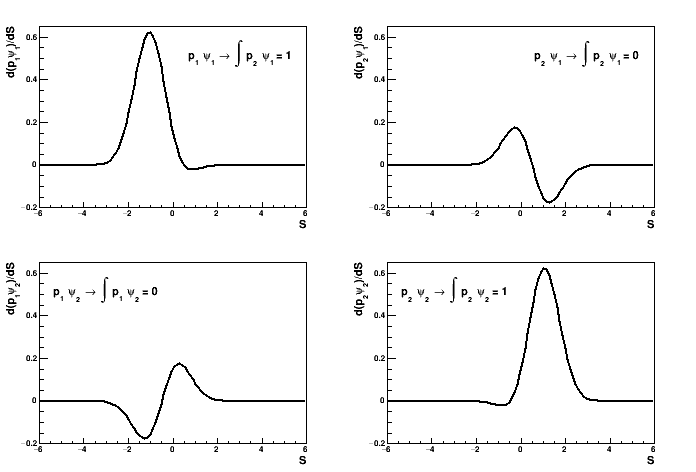
\includegraphics[width=0.7\textwidth]{../png/figSPgaus.png}
\caption{Scalar product functions for the two Gaussian responses case ($\Delta_{12} = 2$).}
\label{fig:SPGaus2}
\end{figure}

To verify the effectiveness of the methods we simulated a sample of $10^5$
events distributed on the two classes with relative abundances of 70\% and
30\% respectively.
Therefore, the event signals generated are distributed as shown in
Fig.~\ref{fig:InputGaus2} where a double Gaussian structure is reported.

\begin{figure}[!htb]
\centering
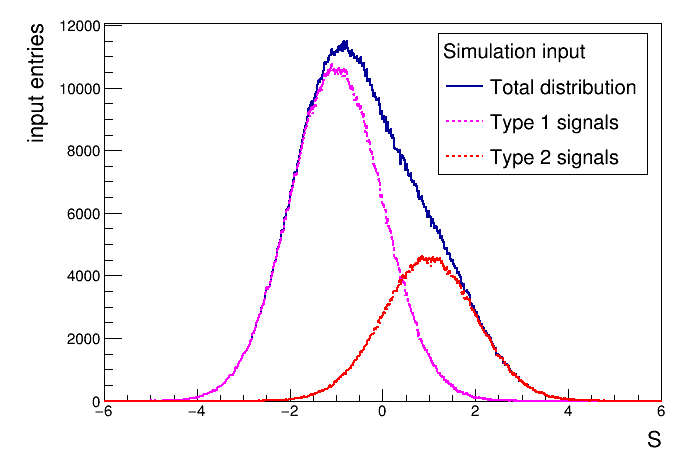
\includegraphics[width=0.7\textwidth]{../png/figInput.png}
\caption{Inputs of the simulation with $\Delta_{12} = 2$ (type 1: 70\%, type 2: 30\%).}
\label{fig:InputGaus2}
\end{figure}

In order to validate the methods the signals generated were processed/counted
for all the events and weighted with the Bayesian probability or
alternativelly with the QM amplitude.
For the Bayesian approach the procedure was iterated in 20 steps with
different set of prior probability. To avoid any bias we started assuming
equal abundances at step 1 and the ones obtained from the previous step
($n-1$) for the n-th step.

In Fig.~\ref{fig:IterGaus2} the results obtained with the two methods are
reported for the case presented and for a similar simulation with a worse
separation between the two classes $\Delta_{12} = 1$.
As it can be noted, while the QM approach returns the correct result at the
first step, the Bayesian appraoch needs more step to reach a convergence to
the truth. The speed of the convergence is high in the first case
($\Delta_{12} = 2$) when a good separation is assumed, while it is quite slow
when the separation is at the level of $1\sigma$.

\begin{figure}[!htb]
\centering
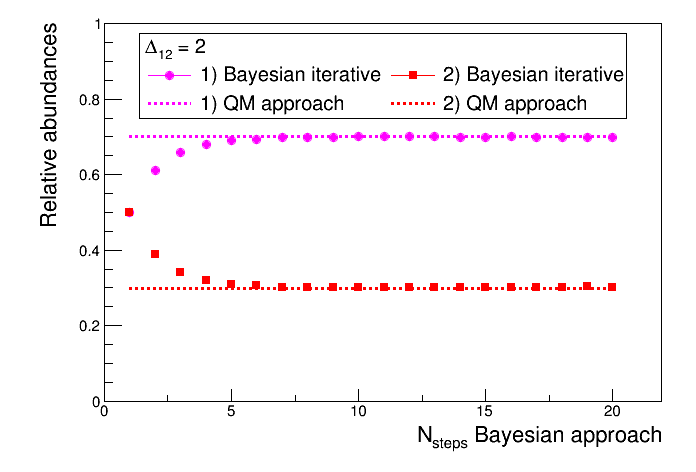
\includegraphics[width=0.45\textwidth]{../png/figIterativeDelta2.png}
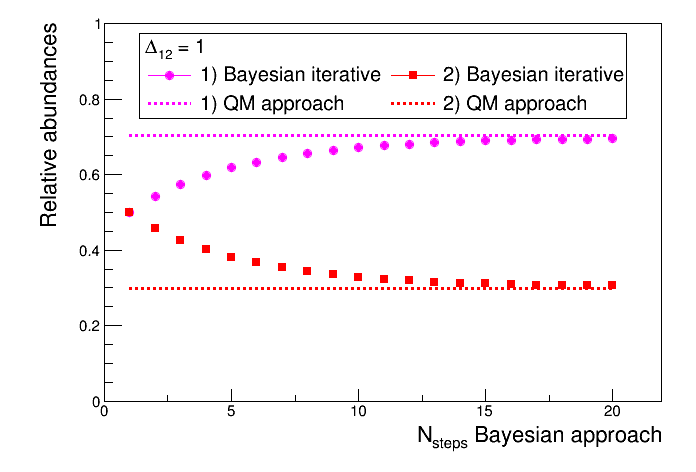
\includegraphics[width=0.45\textwidth]{../png/figIterativeDelta1.png}
\caption{Comparison of the two approaches: results for $\Delta_{12} = 2$ and
  $\Delta_{12} = 1$ cases.}
\label{fig:IterGaus2}
\end{figure}

In any case the two methods are consistent as expected.

\subsection{Characterizing classes using probabilities}
In the previous example we showed that the usage of probabilities as weights
allows to extract the abundances of different classes in a very precise way.
However, the real advantage of such a technique is not in such an operation
because the same result can be achived by simply fitting the signal
distribution with templates derived by the detector response (unfolding).
What is interesting in this novel approach is that the probability is defined
for each single event and it can be used to construct any observable for a
pure event class selection without any additional work.

To give an idea of the powerful of the method we introduced other variables
$x,y$ which descibe some properties of the two event classes.
For simplicity the two variables are defined in the $[0,1]$ range.
The detector response are still defined as in the previous example but in this
case we introduced a dependece of the relative abundances on the variable $x$
as shown in Fig.~\ref{fig:SimEx2}-left.

\begin{figure}[!htb]
\centering
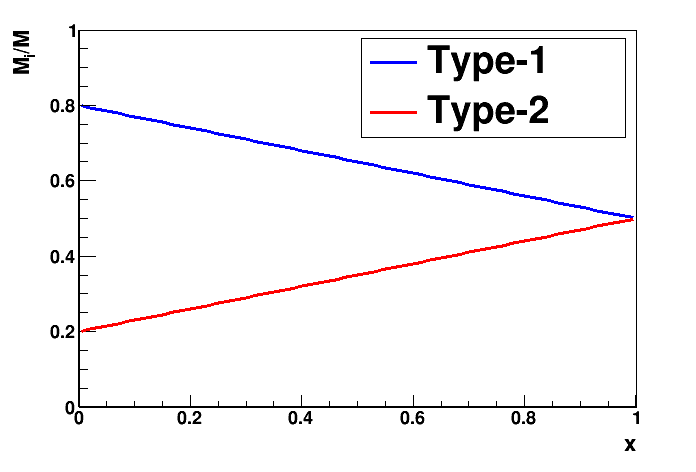
\includegraphics[width=0.3\textwidth]{../png/figAbundances.png}
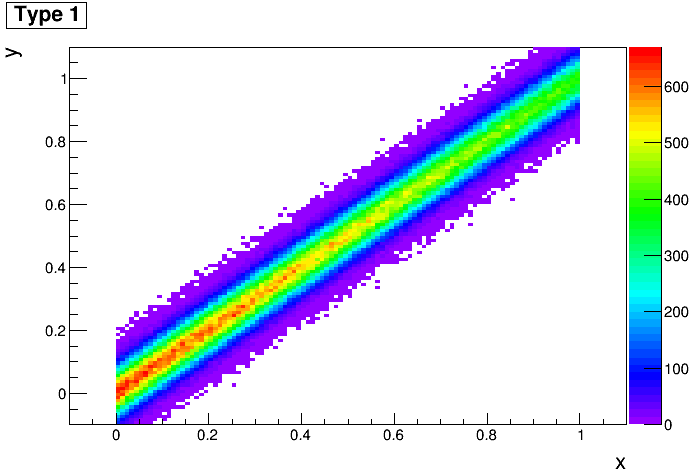
\includegraphics[width=0.3\textwidth]{../png/figType1.png}
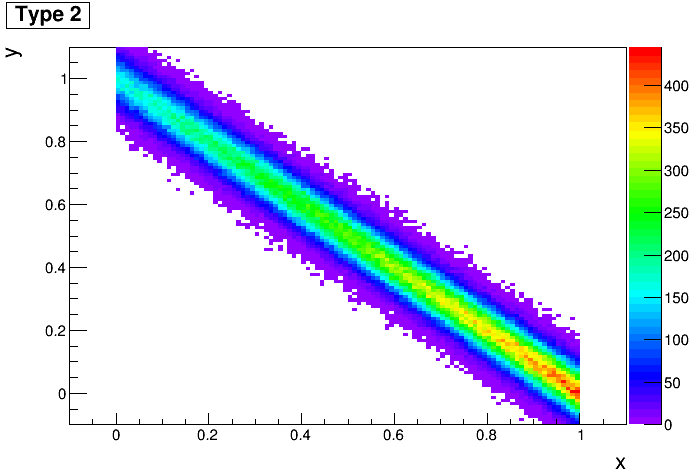
\includegraphics[width=0.3\textwidth]{../png/figType2.png}
\caption{}
\label{fig:SimEx2}
\end{figure}

In addition we introduced a correlation between the $x$ and $y$ variables
which is different for the two classes of events (Fig.~\ref{fig:SimEx2}-right). 
In our data sample the two $x,y$-distributions are merged and can be
distinguished only via the variable $S$ (Fig.~\ref{fig:InputGaus2}).

It can be shown that the Bayesian probability works only introducing a
dependence of the priors probabilities on both the two new variables
($C_{i}(x,y)$). This is in general a limitation of the method when the
  number of variables we want to work with is large.
For this reason we report only results for the QM method which is independent
of any guess of the abundances.

In Fig.~\ref{fig:RecoEx2} the $x,y$-distribution are reported when using the QM amplitude
to fill histograms.
As it can be noted the two classes of events are fully separated.
There is still a light shadow which has memory of the existence of the other
class and which is due to the statistical fluctuations of the finite
statistics used. In any case it is negligible if the statistics is high enough
as in our case ($10^{6}$ events).

\begin{figure}[!htb]
\centering
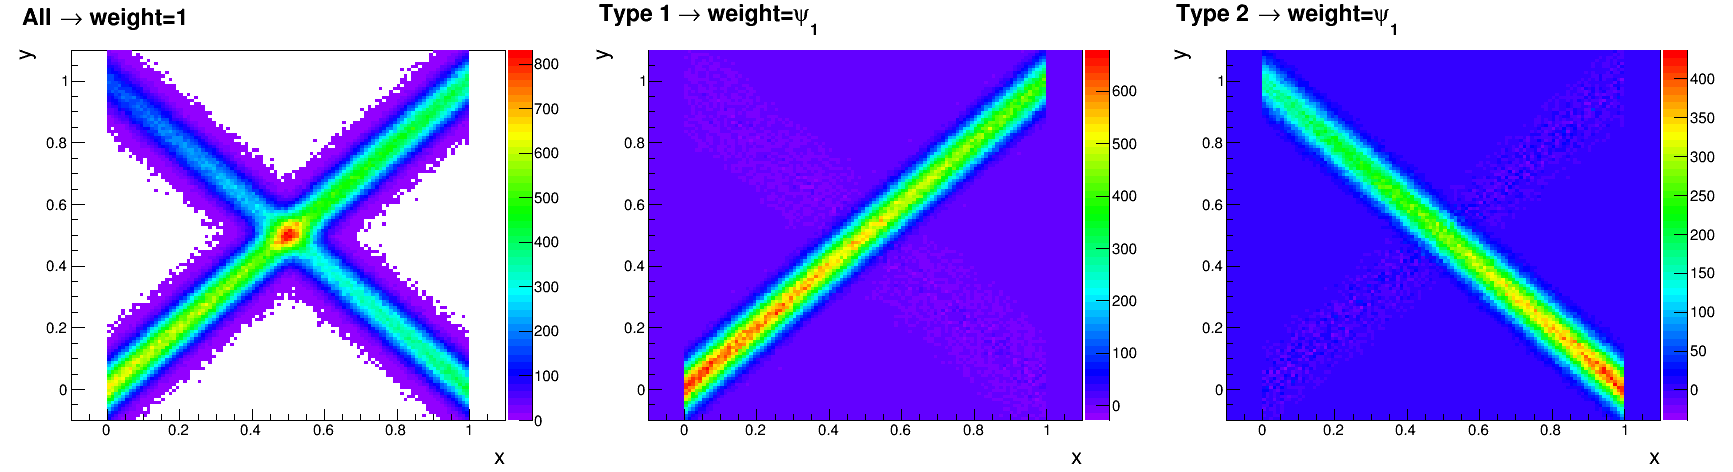
\includegraphics[width=0.8\textwidth]{../png/figRecoCorr.png}
\caption{}
\label{fig:RecoEx2}
\end{figure}

This last result demonstrated that if the amplitude/probability is properly
defined it is possible to work on the data sample as the different classes were
perfectly separted.


\subsection{Correlations of event pair}

\newpage
